\begin{frame}{Глава 3. Модель контактного взаимодействия}
    \minipage{0.45\textwidth}
        \begin{figure}[htb]
            \centering
            % 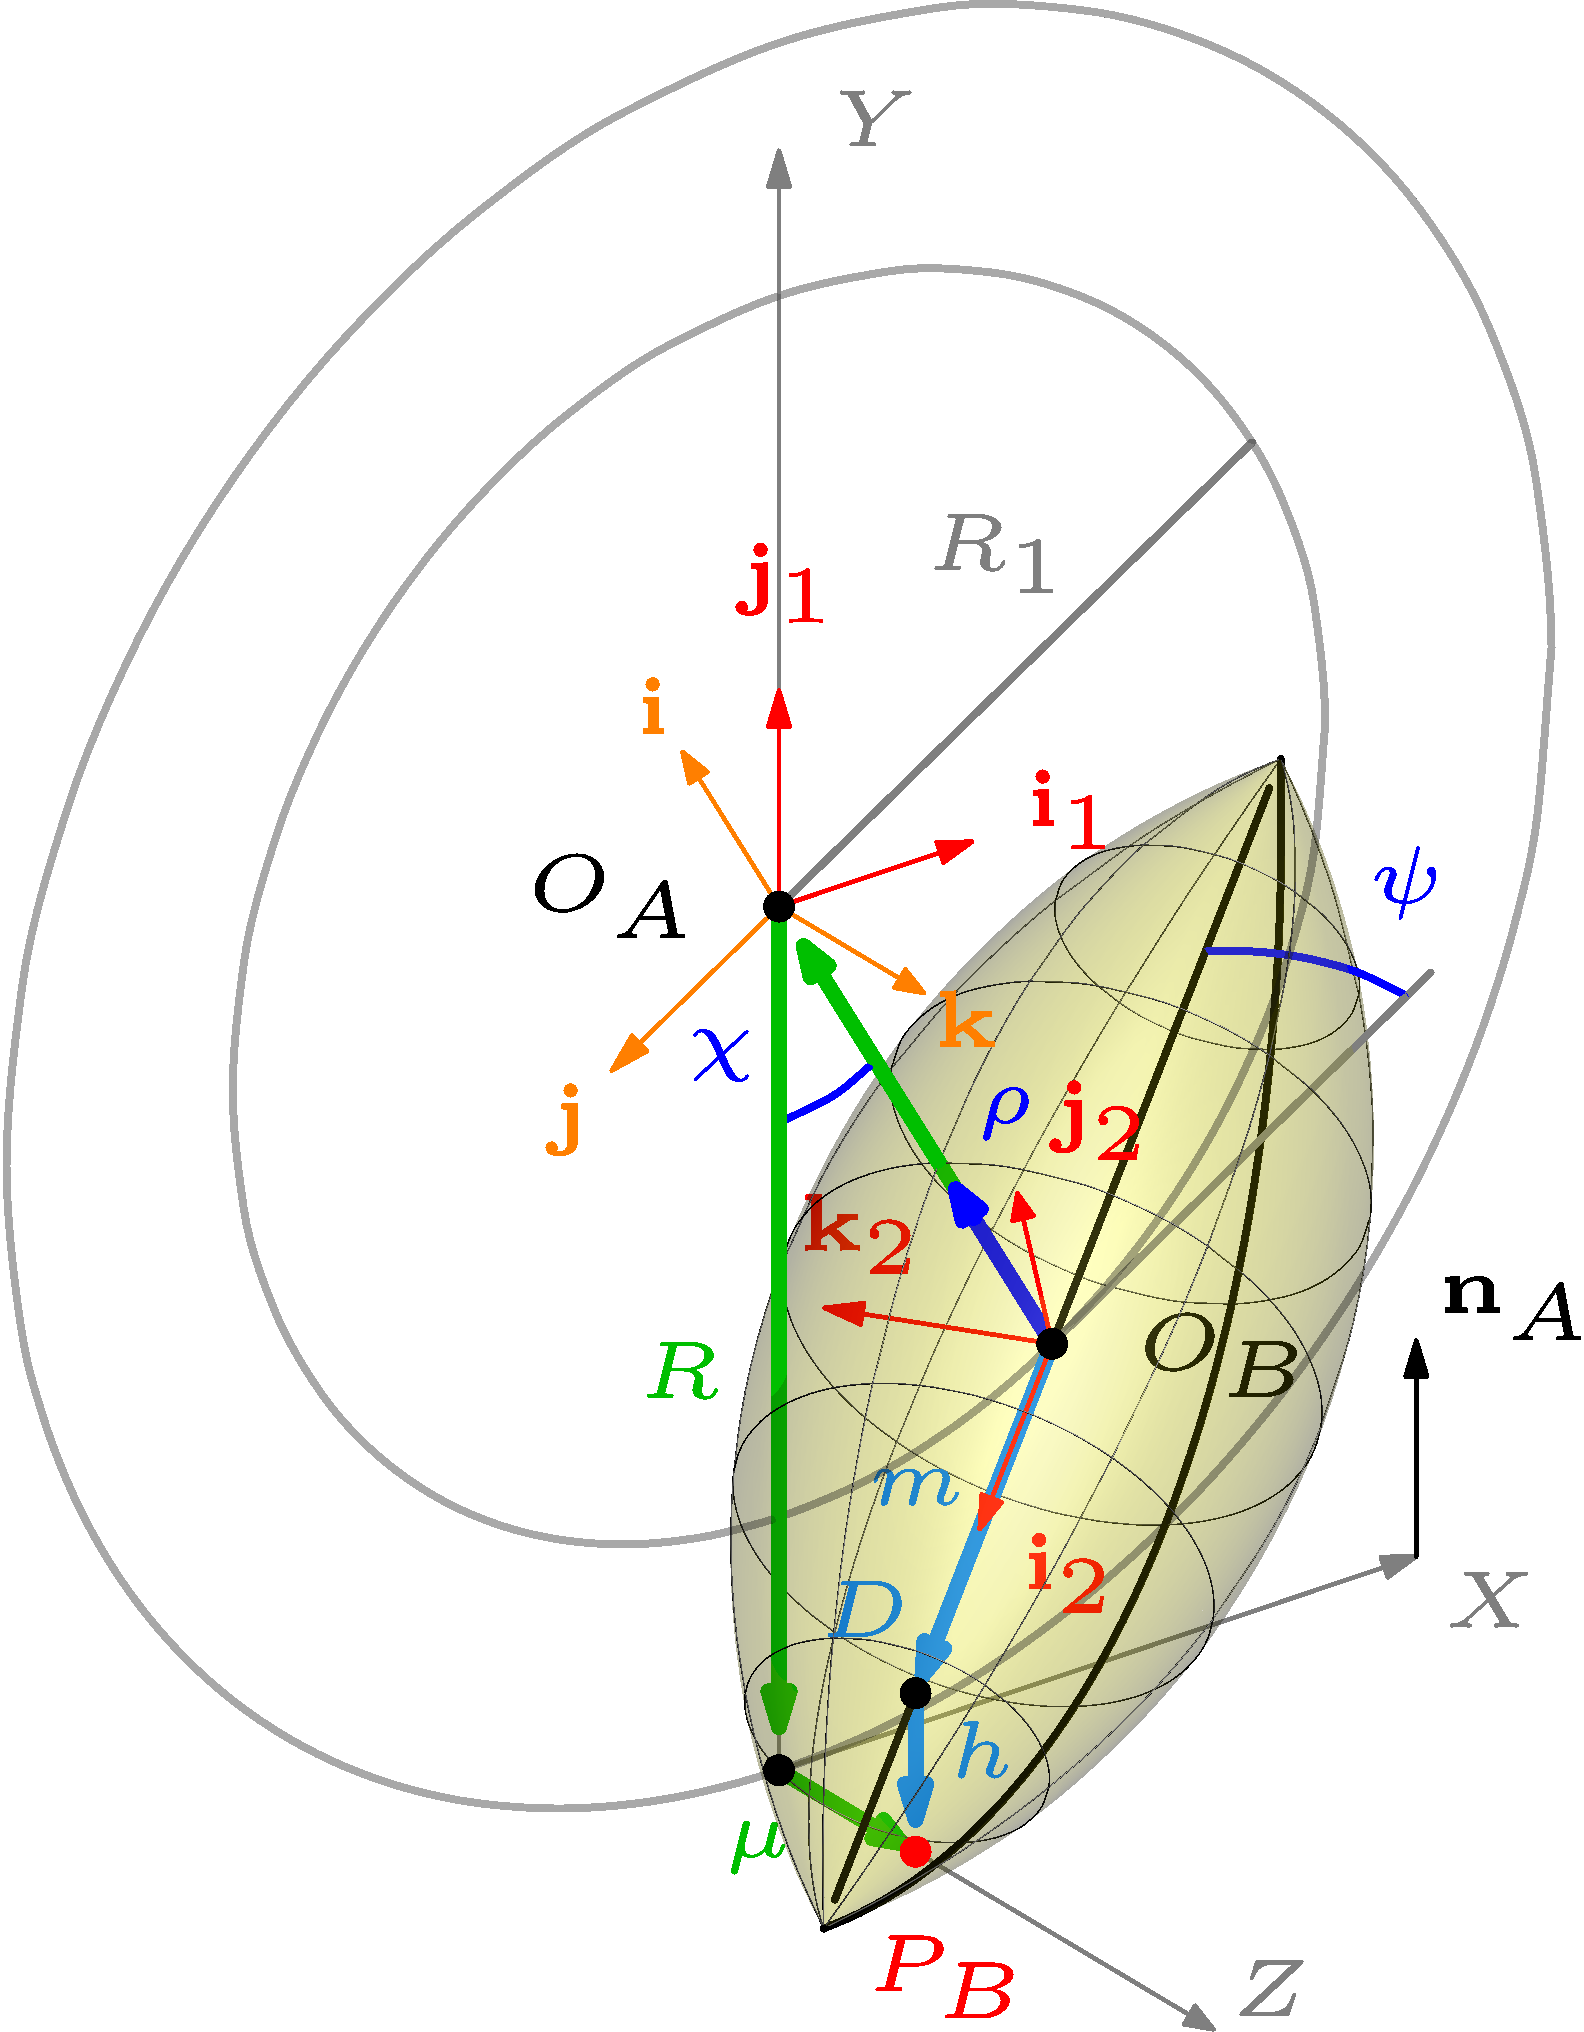
\includegraphics[width=\textwidth]{content/pic/asy/pic_mecanum.png}
            \asyinclude[width=\textwidth]{content/pic/asy/pic_mecanum.asy}
            \label{ContactScheme}
        \end{figure}
    \endminipage
    \quad
    \minipage{0.5\textwidth}
        $$ \vec{r}_C = \vec{r}_K + r\vec{s} - l\vec{e}_z + \lambda\vec{k}_1 $$
        $$ \lambda = \ddfrac{\left(r\vec{s} - l\vec{e}_z\right)\cdot\vec{k}_2}{ \vec{k}_1\cdot\vec{k}_2} $$
        $$ \vec{v}_C = \vec{v}_K + [ \vec{\omega}_{\text{рол}}, \overrightarrow{KC} ] $$
        Ролик находится в контакте $\iff$ $\vec{s} \cdot \vec{e}_z < \cos\ddfrac{\pi}{n} $ и $ z_C < l $. Тогда используются уравнения:
        $$ \vec{v}_C \cdot \vec{e}_z = 0 $$
        $$ \vec{R}_{\text{к}} = \vec{F}_{\text{тр}} + N\vec{e}_z $$
        Иначе $ \vec{R}_{\text{к}} = \vec{0} $
    \endminipage
\end{frame}